\section{Hardware Components and Constructions}

.. generic description and diagram .. (Chris)

\subsection{VXS/VME crates and CPU units (Abbott)}

\subsection{Trigger Disctribution system modules (TS, TD. TI)(William)}
	
\subsection{Signal Distribution module (SD)(Cody)}

\subsection{Flash ADC module (FADC250)(Hai)}

\subsection{Discriminator module (DSC2)(Ben)}

\subsection{TDC modiles (v1190/v1290)(Sergey)}

\subsection{Drift Chamber Discriminator/TDC module (DCRB)(Ben)}

\subsection{VXS Silicon Readout Module (VSCM)}

The CLAS12 Silicon Vertex Tracker (SVT) detector front-end utilizes the data driven FSSR2 ASIC for digitization. The VXS Silicon Readout Module (VSCM) Fig.~\ref{fig:vscm_board} was designed to interface the FSSR2 based front-end to the CLAS12 DAQ system. This system is capable of reading out all 33,792 SVT channels in 3 VXS crates.

\begin{figure}[hbt]
	\centering
	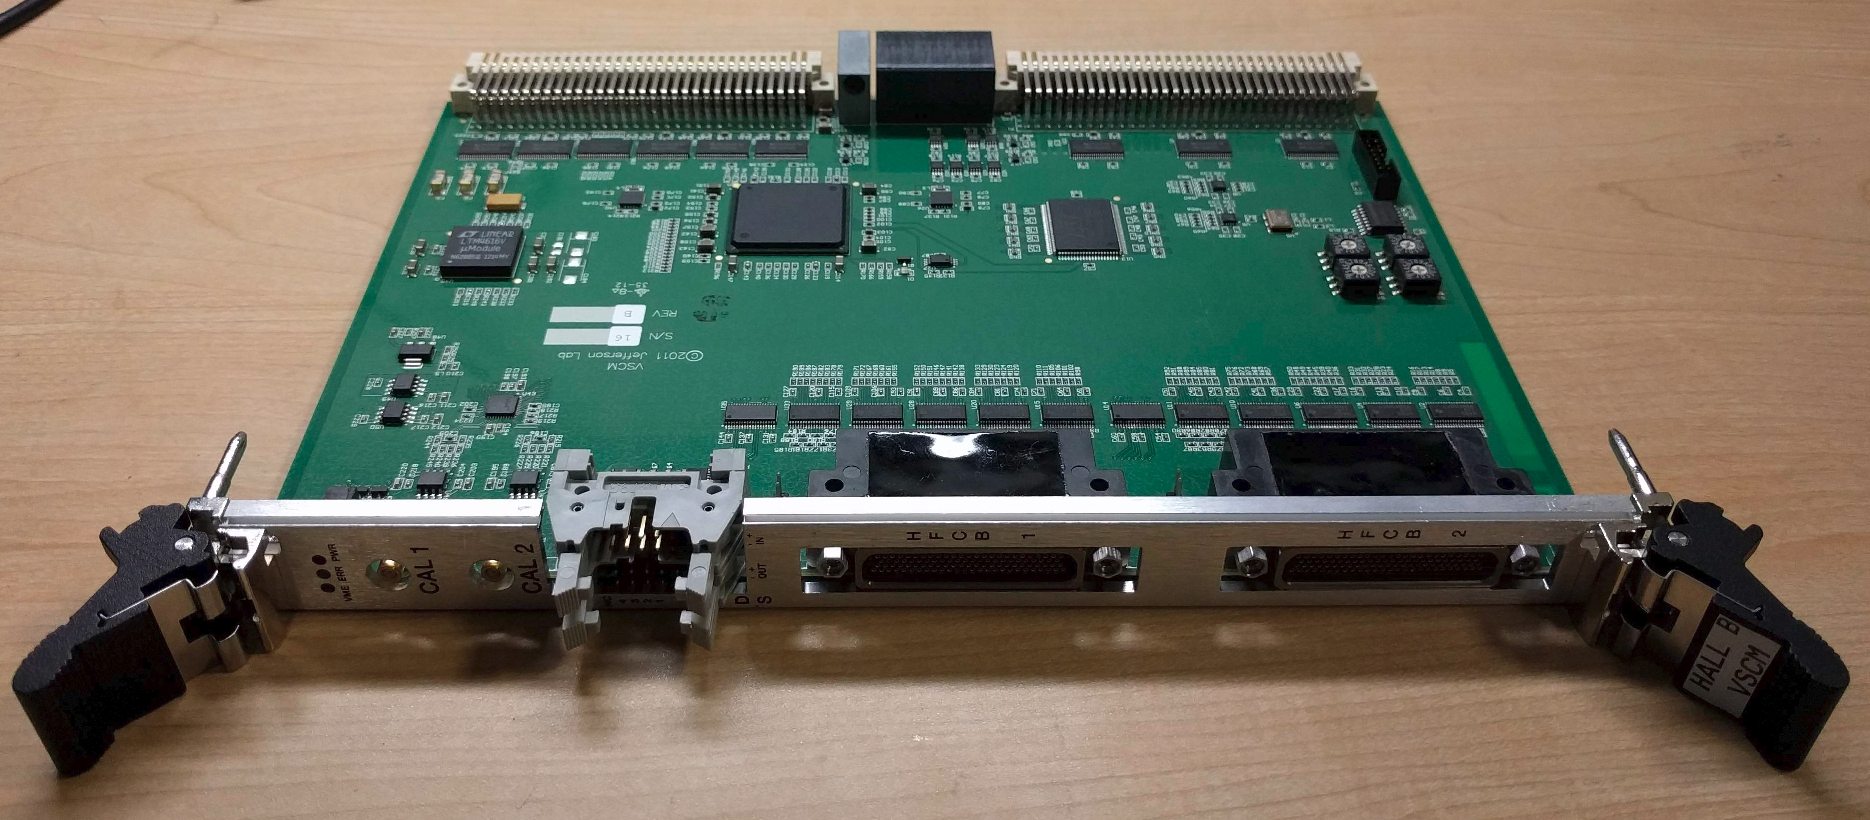
\includegraphics[width=1.0\columnwidth,keepaspectratio]{img/vscm_board.png}
	\caption{VXS Silicon Readout Module (VSCM)}
	\label{fig:vscm_board}
\end{figure}

The main features of the VSCM include:

\begin{itemize}
	\item Receives 8 FSSR2 streams, each at 840Mbps
	\item De-randomizes hits into an 8$\mu$s buffer
	\item 512k multi-hit, multi-event buffer
	\item Supports $>$1MHz trigger rate
	\item Programmable amplitude charge injector
	\item 1ns resolution time-to-digital converter (TDC)
	\item Per channel hit scaler
	\item FSSR2 synchronization, status, and control
\end{itemize}

The VSCM deserializes the FSSR2 streams checking for errors and decoding the hits, which are stored in an 8$\mu$s circular memory. The hits are not guaranteed to be time ordered, so the timestamp and channel number are used to form the circular memory address (rather than storing in the order received). The VSCM also implements an 8 channel 1ns time-to-digital converter (TDC) which measures the logic OR of hits from each FSSR2 ASIC. This high time resolution is significantly better than the FSSR2 serial stream hit time resolution and is required for improved out-of-time hit rejection. The L1A trigger signal time is used to look back a fixed amount of time and extract a time window of hits from the circular memory, which correspond to the physics event. Non-zero hits are as assembled as an event and buffered in an 2MByte external RAM which is readout through the VME bus using the 2eSST protocol at 200MB/s.

The event data contains primarily two hit word types that together provide high time resolution and spatial hit resolution while keeping the front-end complexity low.

\begin{center}
	Low time resolution hit word\\
	\begin{tabular}{| l | l |}
		\hline \hline
		Property	& Description		\\
		\hline
		Hit Time	& 128ns resolution	\\
		Channel		& 0-1023 strip Id	\\
		Charge		& 0-7 threshold		\\
		\hline \hline
	\end{tabular}
\end{center}

\begin{center}
	High time resolution hit word\\
	\begin{tabular}{| l | l |}
		\hline \hline
		Property	& Description		\\
		\hline
		Hit Time	& 1ns resolution	\\
		Channel		& 0-7 chip Id		\\
		\hline \hline
	\end{tabular}
\end{center}

Fig.~\ref{fig:vscm_blockdiagram} shows the hardware block diagram of the module. Essentially a single low-cost Xilinx Spartan 6 FPGA was to implement the deserialization, buffering, event-building, monitoring, front-end configuration, time-to-digital conversion and monitoring.

\begin{figure}[hbt]
	\centering
	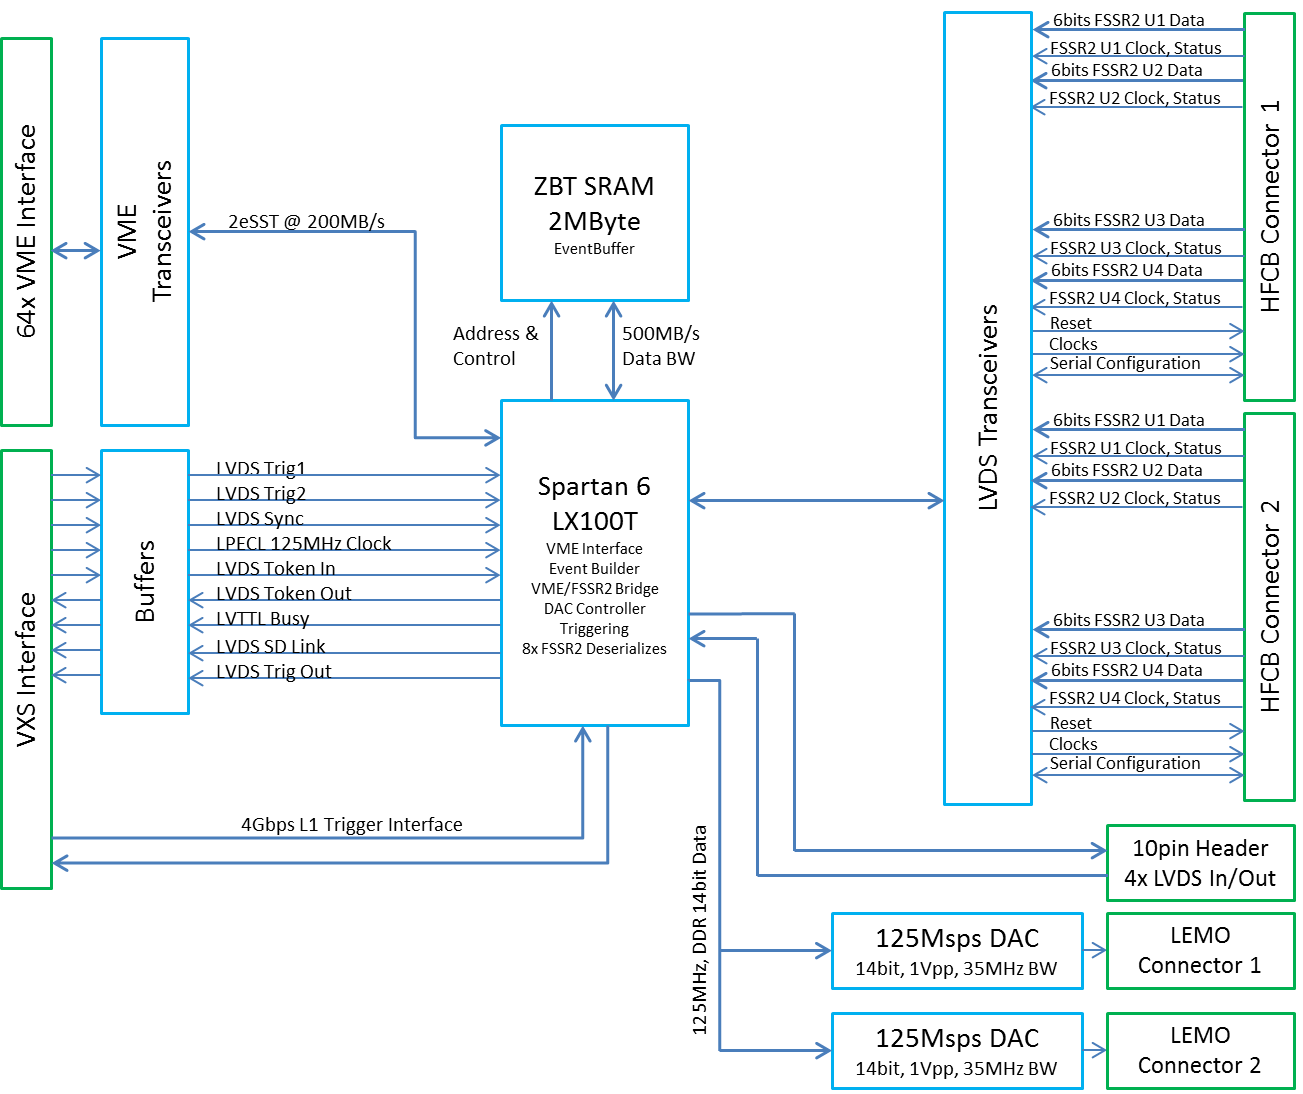
\includegraphics[width=1.0\columnwidth,keepaspectratio]{img/vscm_blockdiagram.png}
	\caption{VSCM Hardware Diagram}
	\label{fig:vscm_blockdiagram}
\end{figure}


\subsection{SSP board as fiber readout module(Ben)}
